\documentclass[10pt,ngerman]{beamer}

\usepackage[ngerman]{babel}

\usetheme[progressbar=frametitle]{metropolis}
\usepackage{appendixnumberbeamer}

\usepackage[utf8]{inputenc}

\usepackage{csquotes}

\usepackage[bibencoding=utf8,
			sortlocale=de,
			style=numeric,
			pagetracker=true,
			autocite=inline,
			backrefstyle=three+,
			date=short,
			sorting=nty,
			backend=biber]{biblatex}
\addbibresource{Literaturverzeichnis.bib}
\renewcommand\bibname{Literaturverzeichnis}

\usepackage{booktabs}
\usepackage[scale=2]{ccicons}

\usepackage{xcolor, soul}
\definecolor{codebackground}{rgb}{0.95, 0.95, 0.92}
\definecolor{Black}{rgb}{0, 0, 0}
\definecolor{sqlpurple}{RGB}{201, 53, 84}
\definecolor{bashred}{RGB}{178, 34, 34}
\definecolor{cicdlila}{RGB}{135, 103, 218}
\definecolor{darkgreenshade}{RGB}{0, 153, 153}
\definecolor{bluekeywords}{rgb}{0.13,0.13,1}
\definecolor{greencomments}{rgb}{0,0.5,0}


\usepackage{graphicx}

% Fuer Notes neben den Folien
\usepackage{pgfpages}
\setbeameroption{show notes on second screen}

\usepackage{siunitx}
\sisetup{
  locale = DE ,
  detect-all
}

\usepackage{tikz}
\definecolor{myblue}{HTML}{92dcec}
\usepackage{smartdiagram}
\usesmartdiagramlibrary{additions} % required in the preamble
\usetikzlibrary{arrows} % required in the preamble

\usepackage{listings}
\lstdefinestyle{MyLatexStyle} {
  frame=tb, % hrule above and below
  keepspaces=true,
  breaklines=true,
  columns=flexible,
  basicstyle=\tt\scriptsize,
  escapeinside={<@}{@>} 
  backgroundcolor=\color{codebackground},
  showstringspaces=false,% for escapin
  language=[LaTeX]TeX,
  keywordstyle=\color{blue},
  identifierstyle=\color{magenta},
  stringstyle=\color{red},
  commentstyle=\color{teal},
  gobble=4
}


\lstloadlanguages{Python}
\lstdefinestyle{MyPythonStyle}{
  backgroundcolor=\color{codebackground},
  basicstyle=\ttfamily,
  breaklines=true,
  columns=flexible,
  commentstyle=\color{teal},
  escapeinside={<@}{@>}, % for escaping
  firstnumber=1,
  flexiblecolumns,
  frame=tb, % hrule above and below
  gobble=-4,
  keepspaces=true,
  keywordstyle={\color{mSybilaRed}},
  keywordstyle=[1]{\color{mSybilaRed}},
  keywordstyle=[2]{\color{darkgreenshade}},
  language=Python,
  morekeywords=[1]{True, as},
  morekeywords=[2]{Queue, EnvConfig, initialize_env, Publisher, connect, get_site_id, empty, get, data_hydration, publish, sleep, Exception},
  numbers=left, % {none, left, right}
  numbersep=5pt,
  numberstyle=\scriptsize\color{black},
  showstringspaces=false,
  stringstyle=\color{darkgreenshade},
  xleftmargin=5.0ex
}

\lstloadlanguages{[Sharp]C}
\lstdefinestyle{cSharpStyle}{
  backgroundcolor=\color{codebackground},
  basicstyle=\ttfamily,
  breaklines=true,
  columns=flexible,
  commentstyle=\color{greencomments},
  escapeinside={<@}{@>}, % for escaping
  firstnumber=1,
  flexiblecolumns,
  frame=tb, % hrule above and below
  gobble=-4,
  keepspaces=true,
  keywordstyle={\color{bluekeywords}},
  keywordstyle=[2]{\color{mSybilaRed}},
  language=[Sharp]C,
  morekeywords=[2]{PAMESANContext, RawData},
  numbers=left, % {none, left, right}
  numbersep=5pt,
  numberstyle=\scriptsize\color{black},
  showstringspaces=false,
  stringstyle=\color{mSybilaRed},
  xleftmargin=5.0ex
}

\lstloadlanguages{SQL}
\lstdefinestyle{sql-style}{
  backgroundcolor=\color{codebackground},
  basicstyle=\texttt\tiny,
  breaklines=true,
  columns=flexible,
  commentstyle=\color{teal},
  escapeinside={<@}{@>}, % for escaping
  firstnumber=1,
  flexiblecolumns,
  frame=tb, % hrule above and below
  gobble=-4,
  keepspaces=true,
  keywordstyle=\color{sqlpurple},
  language=SQL,
  morekeywords={datetime, nvarchar, REFERENCES, uniqueidentifier, varbinary},
  numbers=left, % {none, left, right}
  numbersep=5pt,
  numberstyle=\scriptsize\color{black},
  showstringspaces=false,
  stringstyle=\color{sqlpurple},
  xleftmargin=5.0ex
}

\lstloadlanguages{Bash}
\lstdefinestyle{bash-style}{
  backgroundcolor=\color{codebackground},
  basicstyle=\texttt\tiny,
  belowcaptionskip=-8pt,
  breaklines=true,
  columns=flexible,
  commentstyle=\color{teal},
  escapeinside={<@}{@>}, % for escaping
  firstnumber=1,
  frame=tb, % hrule above and below
  gobble=-4,
  keepspaces=true,
  keywordstyle=\color{bashred},
  language=Bash,
  numbers=left, % {none, left, right}
  numbersep=5pt,
  numberstyle=\scriptsize\color{black},
  showstringspaces=false,
  stringstyle=\color{bashred},
  xleftmargin=5.0ex
}


\lstset{literate=%
    {Ö}{{\"O}}1
    {Ä}{{\"A}}1
    {Ü}{{\"U}}1
    {ß}{{\ss}}1
    {ü}{{\"u}}1
    {ä}{{\"a}}1
    {ö}{{\"o}}1
    {~}{{\textasciitilde}}1
}

\usepackage{caption}

%%% Für Quotes %%%
\usepackage{url}
\usepackage[ngerman]{varioref}
\usepackage{hyperref}
\setlength{\parindent}{0em}
\usepackage{cleveref}
\crefname{paragraph}{Abschnitt}{Abschnitt}

\usepackage{xspace}
\newcommand{\themename}{\textbf{\textsc{metropolis}}\xspace}
\definecolor{mSybilaRed}{HTML}{990000}

\setbeamercolor{title separator}{
  fg=mSybilaRed
}

\setbeamercolor{progress bar}{%
  fg=mSybilaRed,
  bg=mSybilaRed!90!black!30
}

\setbeamercolor{progress bar in section page}{
  use=progress bar,
  parent=progress bar
}

\setbeamercolor{alerted text}{%
  fg=mSybilaRed
}

\makeatletter
\setlength{\metropolis@titleseparator@linewidth}{2pt}
\setlength{\metropolis@progressonsectionpage@linewidth}{2pt}
\setlength{\metropolis@progressinheadfoot@linewidth}{2pt}
\makeatother


\title{Entwicklung von PaMesAn}

% \titlegraphic{\hfill\includegraphics[height=2.5cm]{pictures/python-logo.png}}

%\titlegraphic{\hfill\includegraphics[height=2.5cm]{pictures/LaTeX_logo.png}}
%\titlegraphic{\hfill\includegraphics[height=0.6cm]{sybila-logo/new.png}}
%\titlegraphic{\hfill\includegraphics[height=0.6cm]{sybila-logo/old.png}}
%\titlegraphic{\hfill\includegraphics[height=0.6cm]{sybila-logo/old-flat.png}}

\date{11.01.2023}
\author{Johannes Leyrer}
\institute{FLYERALARM - Azubi-Nr.: 468322}

\subtitle{Implementierung eines neuen Systems zur Erfassung von Versandverpackungen mit Hilfe von Bild- und Sensordaten zur Erfüllung der Novelle des Verpackungsgesetzes}
%\institute{Center for modern beamer themes}
% \titlegraphic{\hfill
\includegraphics[height=0.5cm]{pics/FA_Logo-WM_M_P_1C.pdf}}

\setbeamertemplate{footline}
{
  \leavevmode
  \hbox{
  \begin{beamercolorbox}[wd=.15\paperwidth,ht=2.25ex,dp=1ex,center]{title in head/foot}
    \usebeamerfont{author in head/foot}{Leyrer - 468322}
  \end{beamercolorbox}

  \begin{beamercolorbox}[wd=.7\paperwidth,ht=2.25ex,dp=1ex,center]{author in head/foot}
    \usebeamerfont{author in head/foot}\insertshorttitle
  \end{beamercolorbox}

  \begin{beamercolorbox}[wd=.15\paperwidth,ht=2.25ex,dp=1ex,center]{title in head/foot}
    \insertframenumber{} / \inserttotalframenumber
  \end{beamercolorbox}
  }
}

\begin{document}

\maketitle

\note[itemize]
{
  \item{Guten Morgen}
  \item{Johannes Leyrer}
  \item{Implementierung eines neuen Systems zur Erfassung von Versandverpackungen mit Hilfe von Bild- und Sensordaten zur Erfuellung der Novelle des Verpackungsgesetzes}
  \item{Entwicklung von PaMesAn - Paket-Messungs-Anlage}
}


\begin{frame}{Gliederung}
  \setbeamertemplate{section in toc}[sections]
  \tableofcontents[hideallsubsections]
\end{frame}

\note[itemize]
{
  \item{Projektumfeld}
  \item{Planungsphase}
  \item{Analysephase}
  \item{Entwurf}
  \item{Implementierung}
  \item{Fazit und Ausblick}
}



\section{Projektumfeld}
\begin{frame}[fragile]{FLYERALARM GmbH}
  \centering{\Large{FLYERALARM GmbH}}

  \begin{table}
    \begin{tabular}{lll}
      2002      & $>$ 2000      & $>$ 3 Mio \\
      gegründet & Mitarbeitende & Produkte  \\
    \end{tabular}
  \end{table}

  \note<1->[item]{FLYERALARM GmbH, 2002 gegründet, $>$ 2000 Mitarbeitende und $>$ 3 Mio Produkte}

  \pause

  \begin{itemize}
    \item Eines der größten E-Commerce Unternehmen Deutschlands
          \note<2->[item]{Eines der größten E-Commerce Unternehmen Deutschlands}
          \pause
    \item Führende Online-Druckerei Europas im B2B-Bereich
          \note<3->[item]{Führende Online-Druckerei Europas im B2B-Bereich}
          \pause
    \item Zuständig für Design und Marketing
          \note<4->[item]{Zuständig für Design und Marketing}
          \pause
    \item Erstellung der Druckdaten
          \note<5->[item]{Zustaendig fuer die Erstellung der Druckdaten}
  \end{itemize}
\end{frame}


\begin{frame}[fragile]{FLYERALARM Industrial Print GmbH}
  \centering{\Large{FLYERALARM Industrial Print GmbH}}

  \begin{table}
    \begin{tabular}{lll}
      8         & ca. 1200      \\
      Standorte & Mitarbeitende \\
    \end{tabular}
  \end{table}

  \note<1->[item]{FLYERALARM Industrial Print GmbH (FAIP) an 8 Standorten mit ca. 1200 Mitarbeitenden}

  \pause

  \begin{itemize}
    \item Tochtergesellschaft
          \note<2->[item]{Tochtergesellschaft der FLYERALARM GmbH}
          \pause
    \item Eigene IT-Abteilung
          \note<3->[item]{Eigene IT-Abteilung}
          \pause
    \item Produktion und Versand
          \note<4->[item]{Zustaendig fuer Produktion und Versand}
  \end{itemize}
\end{frame}



\section{Planung}
\begin{frame}[fragile]{Zeitschätzung Projektphasen}
  \begin{tikzpicture}

    \draw (0cm,0cm) -- (9.5cm,0cm);  %Abzisse
    \draw (0cm,0cm) -- (0cm,-0.1cm);  %linkes Ende der Abzisse
    \draw (9.5cm,0cm) -- (9.5cm,-0.1cm);  %rechtes Ende der Abzisse

    \draw (-0.1cm,0cm) -- (-0.1cm,4.5cm);  %Ordinate
    \draw (-0.1cm,0cm) -- (-0.2cm,0cm);  %unteres Ende der Ordinate
    \draw (-0.1cm,4.5cm) -- (-0.2cm,4.5cm) node [left] {h};  %oberes Ende der Ordinate

    \foreach \x in {10,20,...,40}  %Hilfslinien
    \draw[gray!50, text=black] (-0.2 cm,\x * 0.1 cm) -- (9.5 cm,\x * 0.1 cm)
    node at (-0.5 cm,\x * 0.1 cm) {\x};  %Beschriftung der Hilfslinien

    \node at (4.5cm,5cm) {Grobe Zeitplanung};  %Überschrift

    \foreach \x/\y/\country in {0.5/10/Analyse,  %\x ist Anfang der Säulen
        2/8/Entwurf,  %\y ist Höhe der Säulen
        3.5/39/Implementierung,
        5/5/Test,
        6.5/6/Einführung,
        8/12/Dokumentation}
      {
        \draw[fill=mSybilaRed] (\x cm,0cm) rectangle (1cm+\x cm,\y * 0.1 cm) %die Säulen
        node at (0.5cm + \x cm,\y * 0.1 cm + 0.3cm) {\y}; %die Prozente über den Säulen
        \node[rotate=45, left] at (0.6 cm +\x cm,-0.1cm) {\country}; %Säulenbeschriftung
      };

  \end{tikzpicture}
\end{frame}

\note[itemize]
{
  \item{10h Analyse}
  \item{8h Entwurf}
  \item{39h Implementierung}
  \item{5h Test}
  \item{6h Einführung}
  \item{12h Dokumentation}
  \item{Implementierung so gross wegen der Bilderkennung}
}



\section{Analyse}
\begin{frame}[fragile]{Ist-Analyse}
  \textbf{Ist-Analyse}
  \begin{itemize}
    \item Paketgröße und Anzahl werden manuell gepflegt
          \note<1->[item]{Paketgröße und Anzahl werden manuell gepflegt}
          \pause
    \item Neue Anforderungen durch  Verpackungsgesetz
          \note<2->[item]{Es gibt neue Anforderungen durch  Verpackungsgesetz, es reicht nicht mehr, nur noch Gewicht zu melden}
          \pause
    \item Hoher Wartungsaufwand für pflegende Personen
          \note<3->[item]{Hoher Wartungsaufwand}
  \end{itemize}
\end{frame}


\begin{frame}[fragile]{Soll-Analyse}
  \textbf{Soll-Analyse}
  \begin{itemize}
    \item Paketgröße und Anzahl werden automatisch erfasst
          \note<1->[item]{Automatische Erfassung von Paketgröße und Anzahl}
          \pause
    \item Erfüllung der Anforderungen durch Verpackungsgesetz
          \note<2->[item]{Grundlage fuer Anforderungen fuer Verpackungsgesetzes erfuellen: Abmessungen, Gewicht, Materialart, Empfaengerland}
          \pause
    \item Wartungsaufwand minimieren durch automatische Erfassung
          \note<3->[item]{Wartungsaufwand minimieren}
  \end{itemize}
\end{frame}


\begin{frame}[fragile]{Angebot der Elektro Löther GmbH}
  \begin{figure}[htpb]
    \centering
    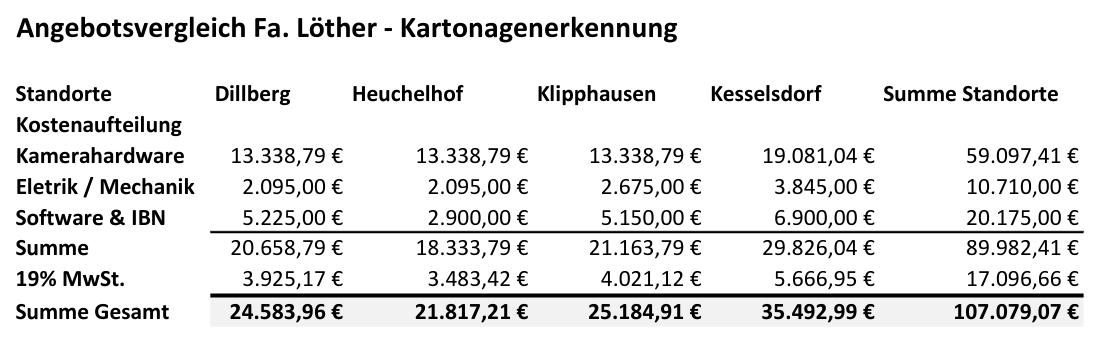
\includegraphics[width=1\textwidth]{pics/AngebotLoether.png}
  \end{figure}
\end{frame}

\note[itemize]
{
  \item{Angebote ermittelt}
  \item{Unternehmen Elektro Loether GmbH}
  \item{Kostenvoranschlag fuer 4 Standorte}
  \item{Kesselsdorf 35k Euro}
}


\begin{frame}[fragile]{Kostenverteilung Hardware}
  \begin{table}[htbp]
    \centering
    \begin{tabular}{lr}
      \textbf{Hardware}          & \textbf{Gesamt}         \\ \hline
      ARCELI Shield Board Kit    & \SI{17.99}{€}           \\
      AZDelivery Mega 2560 R3    & \SI{14.99}{€}           \\
      Benewake TF MINI PLUS      & \SI{182.40}{€}          \\
      Microsoft Lifecam Studio   & \SI{42.99}{€}           \\
      item-Systemprofile         & \SI{29.52}{€}           \\
      item-Verbindungsstücke     & \SI{192.00}{€}          \\
      item-Füße                  & \SI{48.00}{€}           \\
      Dell Wyse 5070 Thin Client & \SI{450.00}{€}          \\
      \hline
      \textbf{Gesamtkosten}      & \textbf{\SI{977.89}{€}}
    \end{tabular}
  \end{table}
\end{frame}

\note[itemize]
{
  \item{Eigenentwicklung}
  \item{977,89 Euro Hardware}
}


\begin{frame}[fragile]{Kostenverteilung Personal und Hardware}
  \begin{table}[htbp]
    \centering
    \begin{tabular}{lrrr}
      \textbf{Personal}     & \textbf{Zeit in h} & \textbf{Kosten pro h}          & \textbf{Gesamt}          \\ \hline
      Auszubildender        & 80                 & \SI{6.00}{€} + \SI{15.00}{€}   & \SI{1680.00}{€}          \\
      Teamleitung           & 2                  & \SI{31.50}{€}  + \SI{15.00}{€} & \SI{93.00}{€}            \\
      Teammitglied          & 2                  & \SI{21.50}{€}  + \SI{15.00}{€} & \SI{73.00}{€}            \\
      Haustechnik           & 8                  & \SI{19.00}{€}  + \SI{15.00}{€} & \SI{272.00}{€}           \\ \hline
      \textbf{Gesamtkosten} &                    &                                & \textbf{\SI{2118.00}{€}}
    \end{tabular}
  \end{table}

  \vspace{0.4cm}

  \textbf{Gesamtkosten Personal und Hardware: \SI{3095.89}{€}}
\end{frame}

\note[itemize]
{
  \item{2118 Euro Pesonalkosten}
  \item{Gesamtkosten 3095,89 Euro}
  \item{Etwa 20k - 30k Euro guenstiger in Eigenentwicklung}
  \item{Entscheidung fuer Eigenentwicklung}
}



\section{Entwurf}
\begin{frame}[fragile]{Sensorträger}
  \begin{figure}[htpb]
    \centering
    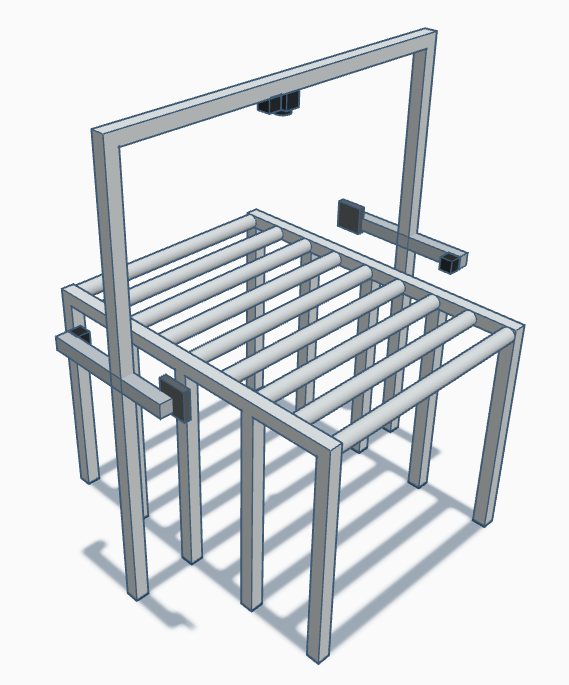
\includegraphics[width=0.6\textwidth]{files/Sensortraeger/Skizze_Sensor_Traeger_3D_verdreht_cropped.png}
  \end{figure}
\end{frame}

\note[itemize]
{
  \item{Entwurf}
  \item{3D Sensortraeger}
  \item{Sensoren seitlich und oben}
  \item{Kamera oben}
}


\begin{frame}[fragile]{Standort}
  \begin{figure}[htpb]
    \centering
    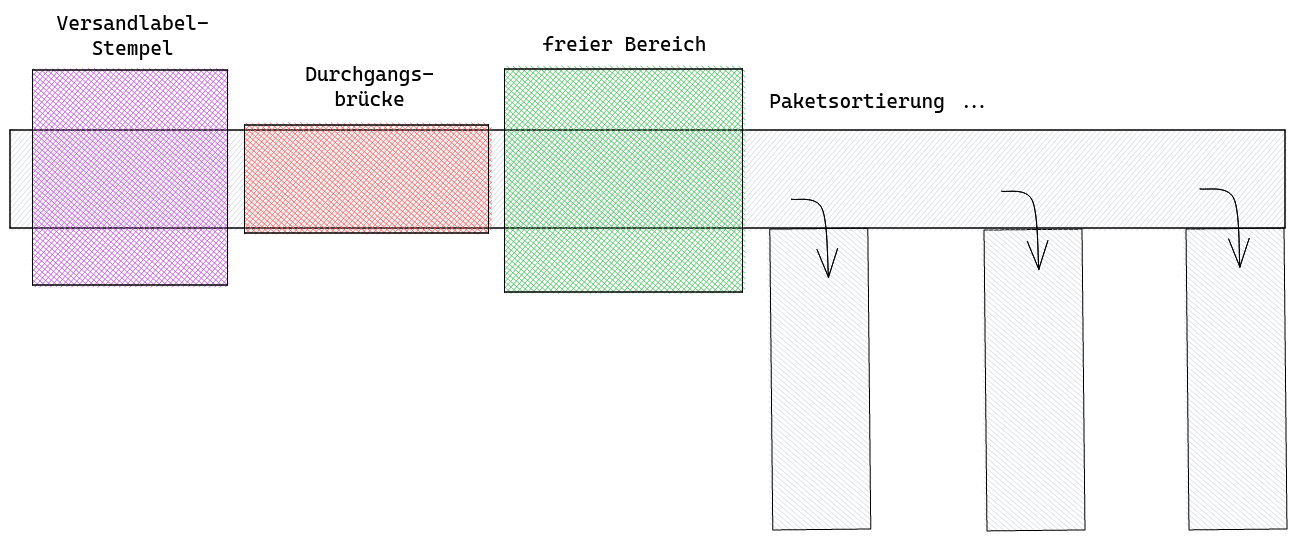
\includegraphics[width=1\textwidth]{pics/Versandanlage.png}
  \end{figure}
\end{frame}

\note[itemize]
{
  \item{Standort}
  \item{Versandanlage}
}


\begin{frame}[fragile]{RabbitMQ}
  \begin{figure}[htpb]
    \centering
    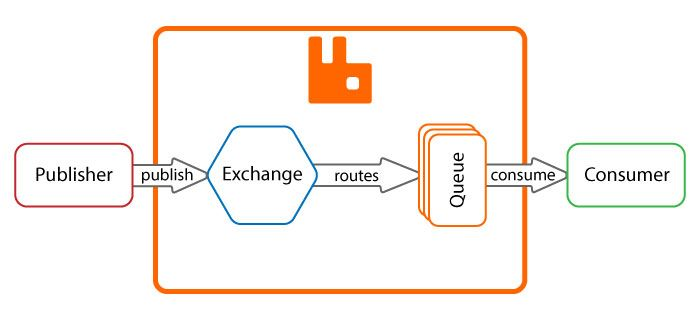
\includegraphics[width=1\textwidth]{pics/rabbitmq-broker.jpg}
  \end{figure}
\end{frame}

\note[itemize]
{
  \item{Microservices-Architektur}
  \item{Kommunikation ueber RabbitMQ}
  \item{RabbitMQ: Open Source Message Broker Software}
  \item{Analog zum Postsystem}
  \item{DANN: RabbitMQ}
  \item{Advanced Message Queuing Protocol (AMQP), binäres Netzwerkprotokoll}
}


\begin{frame}[fragile]{Programmübersicht}
  \begin{figure}[htpb]
    \centering
    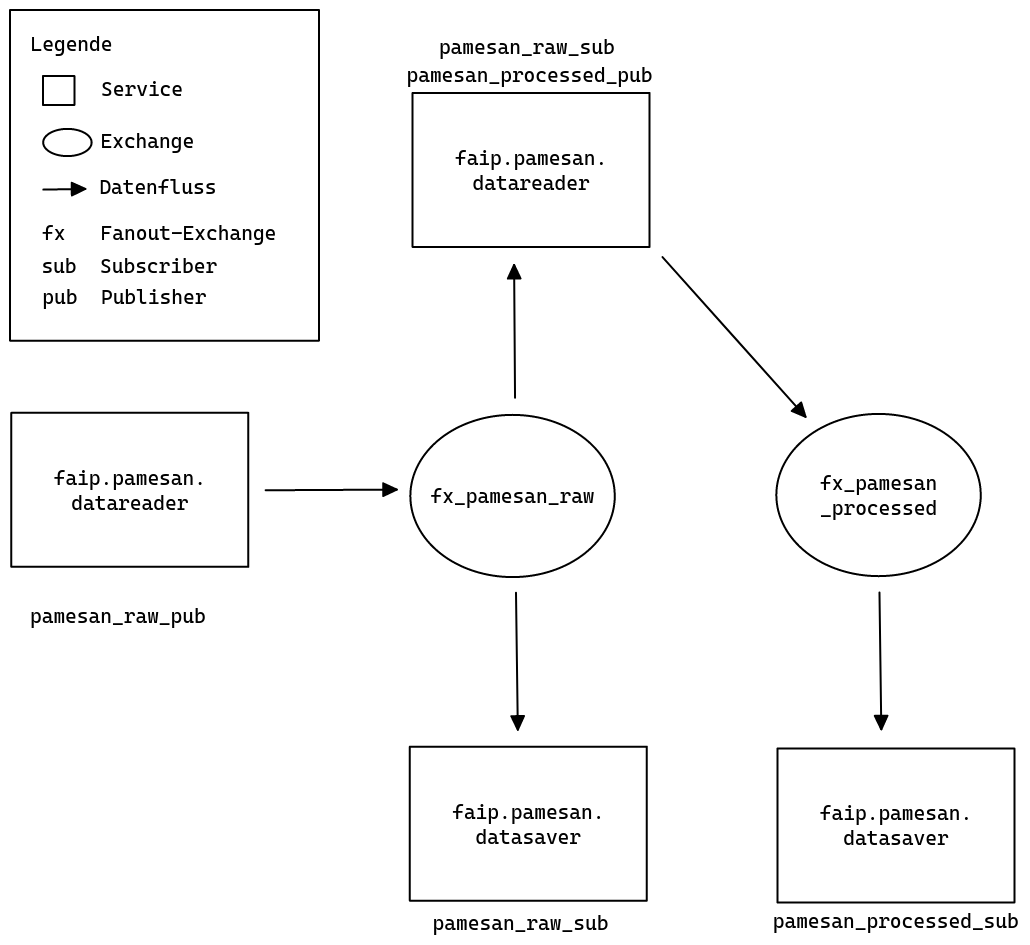
\includegraphics[width=0.75\textwidth]{pics/Architektur.png}
  \end{figure}
\end{frame}

\note[itemize]
{
  \item{4 Services, 2 Exchanges}
  \item{Datenauslese-Service}
  \item{Pamesan-Raw-Exchange}
  \item{Datenspeicherservice}
  \item{Datenverarbeitungsservice}
  \item{Pamesan-Processed-Exchange}
  \item{Datenspeicherservice}
}


\begin{frame}[fragile]{Datenmodell}
  \begin{figure}[htpb]
    \centering
    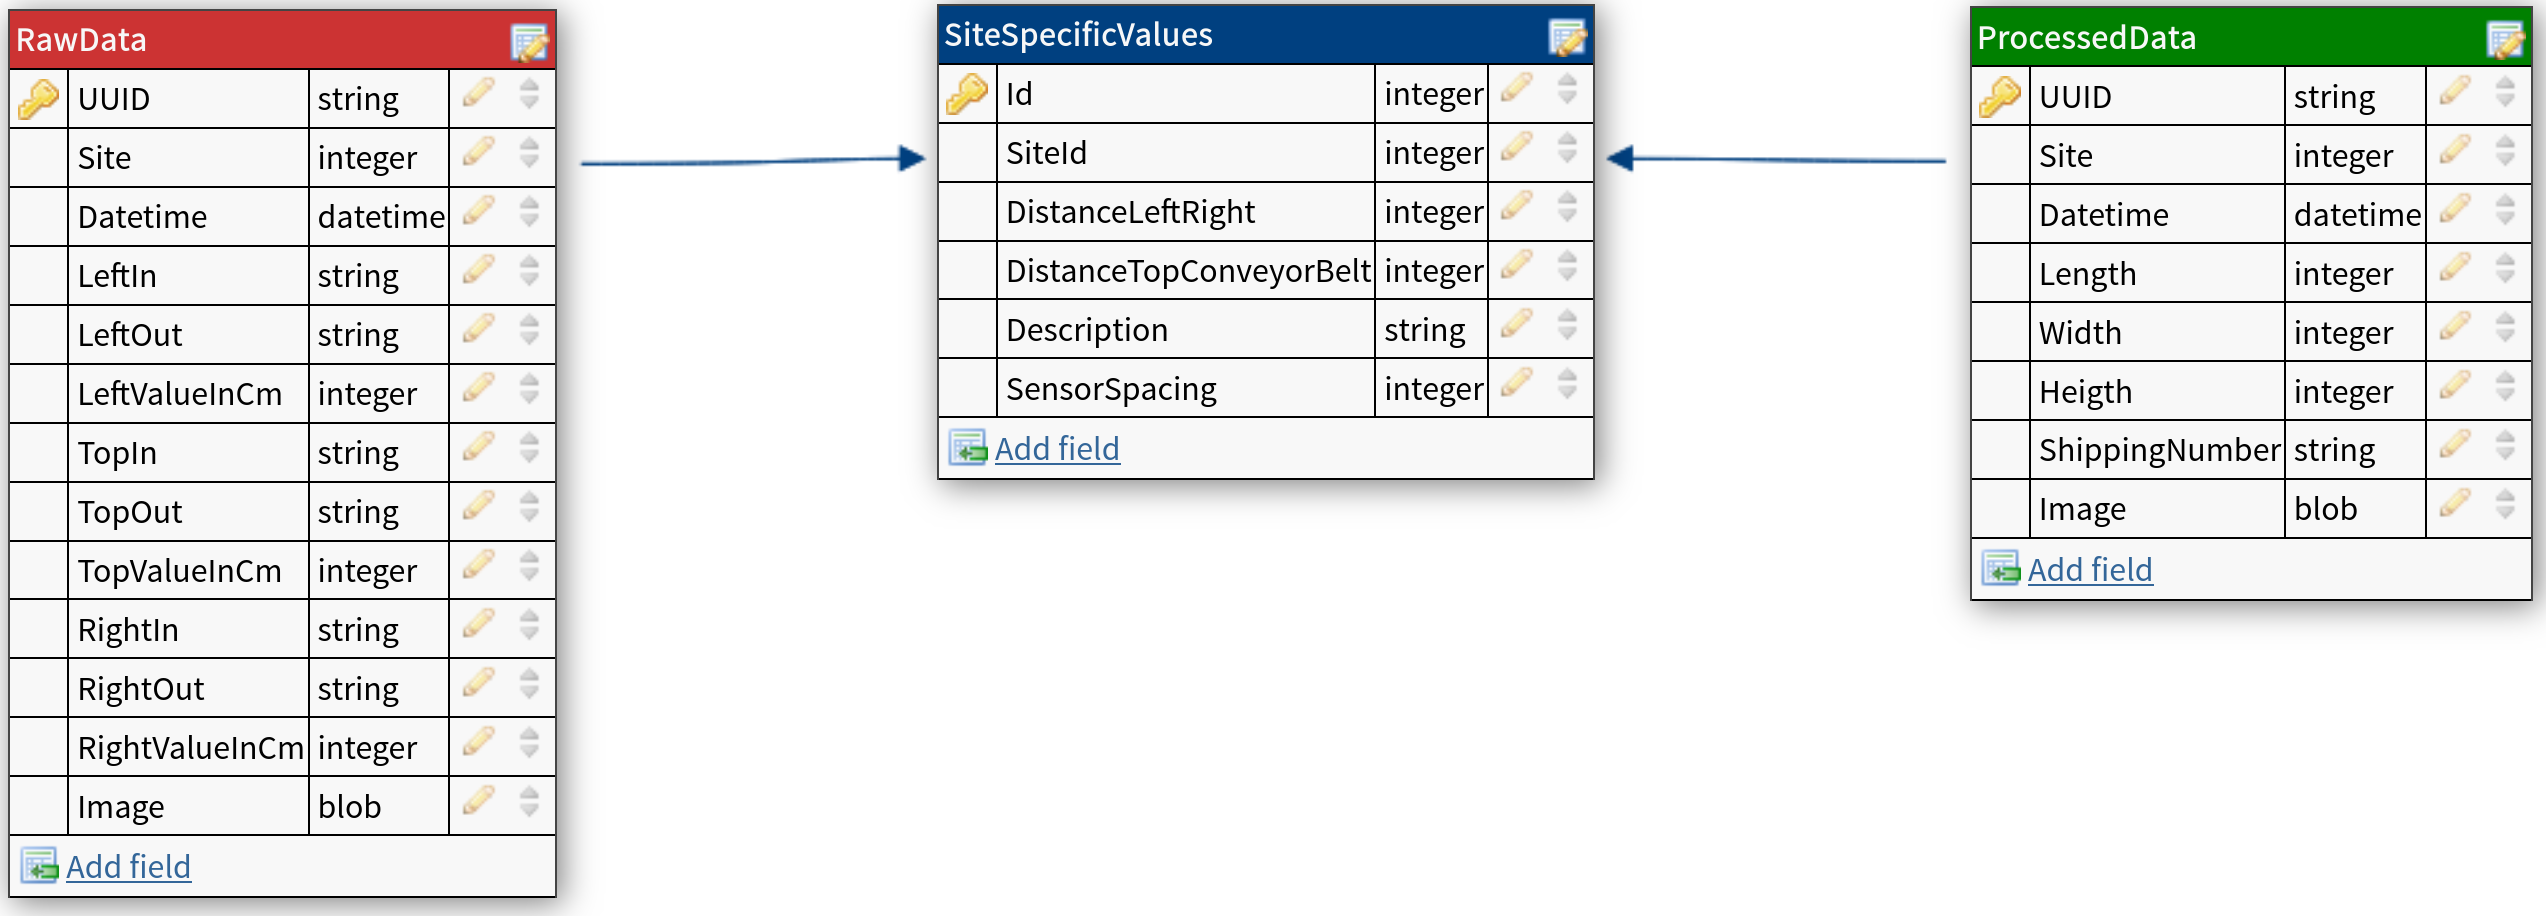
\includegraphics[width=1\textwidth]{pics/Tabellenmodell_schoen.png}
  \end{figure}
\end{frame}

\note[itemize]
{
  \item{MSSQL}
  \item{Tabellenmodell}
  \item{3 Tabellen}
  \item{SiteSpecificValues-Tablle, SensorSpacing}
}



\section{Implementierung}
\begin{frame}[fragile]{Lasersensor und Arduino}
  \begin{minipage}[t]{0.49\textwidth}
    \begin{figure}
      \centering
      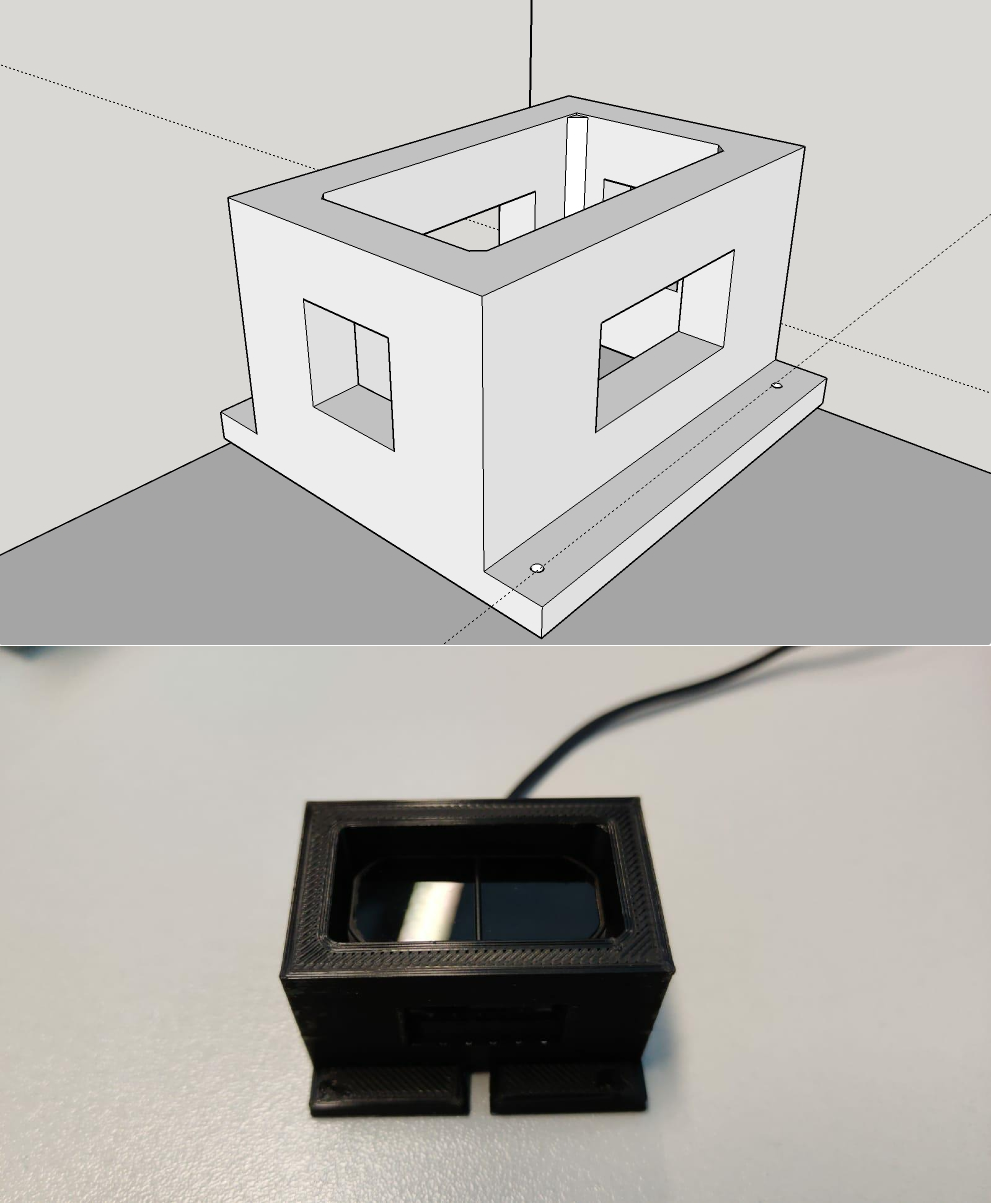
\includegraphics[width=1\textwidth]{pics/thingiverse_3D.png}
    \end{figure}
  \end{minipage}
  \begin{minipage}[t]{0.49\textwidth}
    \begin{figure}
      \centering
      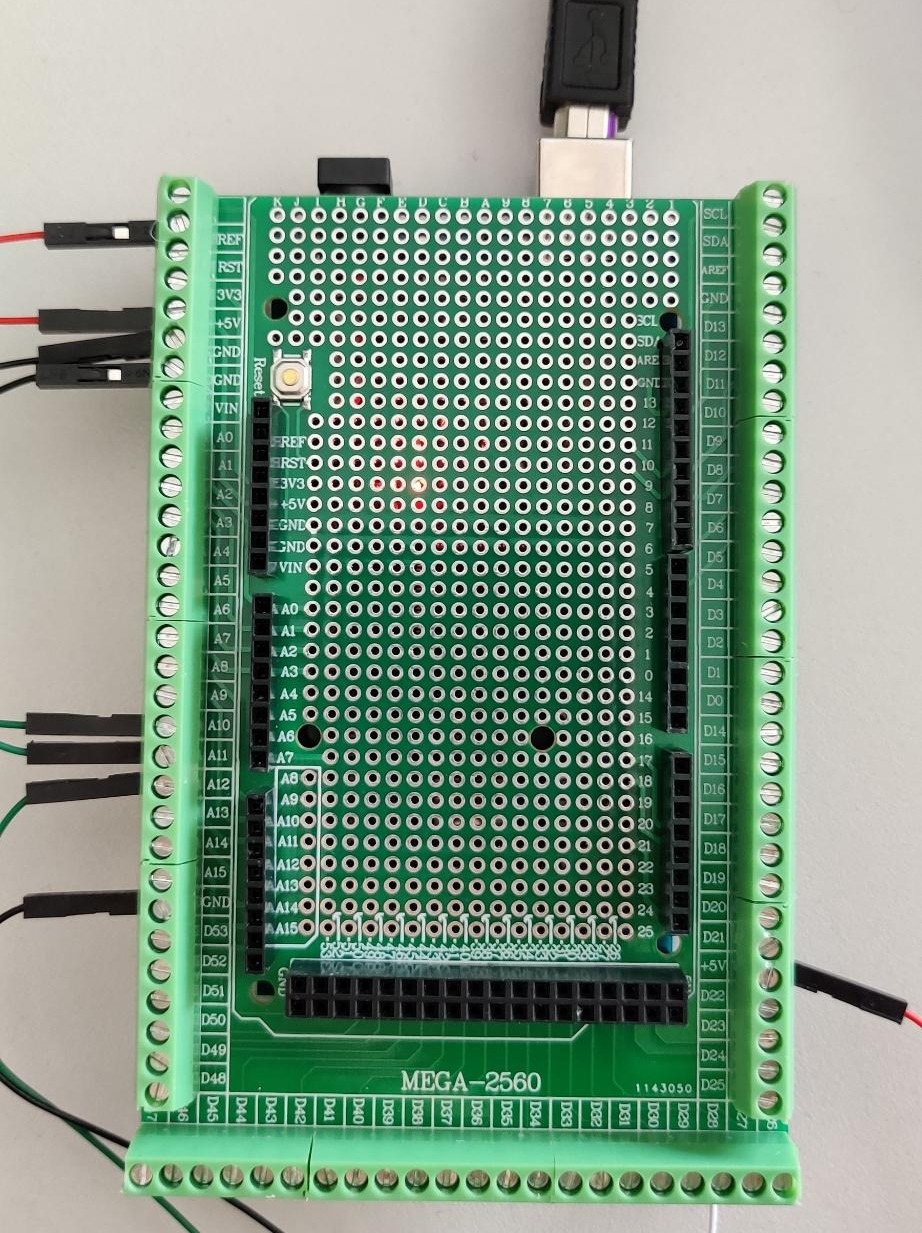
\includegraphics[width=1\textwidth]{pics/Arduino.jpeg}
    \end{figure}
  \end{minipage}
\end{frame}

\note[itemize]
{
  \item{Implementierung}
  \item{Lasersensor}
  \item{3D Druck}
  \item{Minicomputer Arduino mit Shield, gute und sichere Verkabelung}
  \item{Script des Herstellers zum Auslesen der Sensoren}
}


\begin{frame}[fragile]{Umsetzung des Sensorträgers}
  \begin{figure}[htpb]
    \centering
    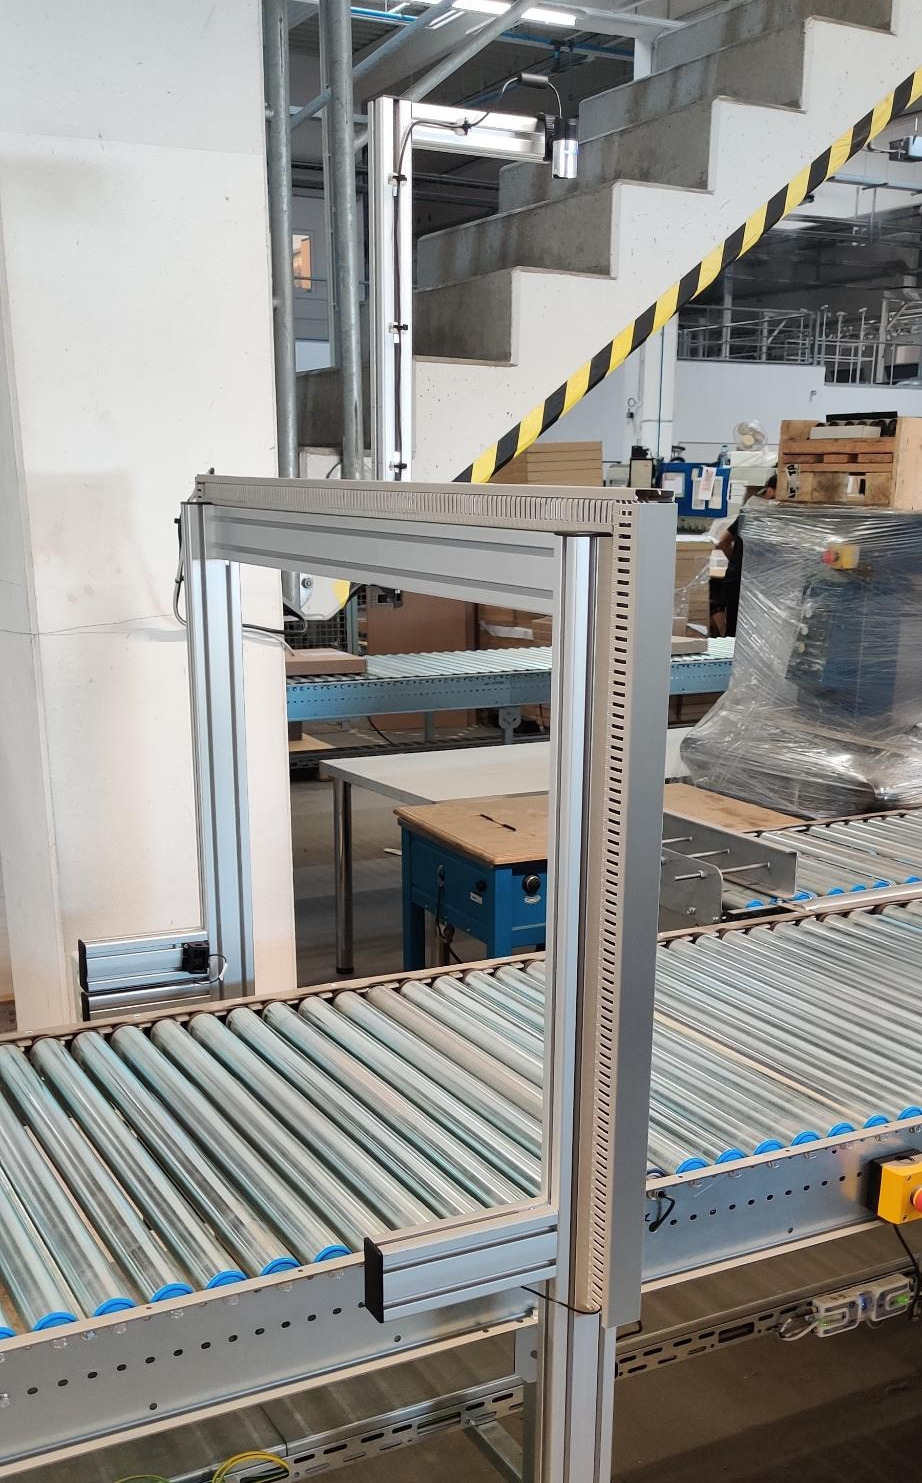
\includegraphics[width=0.45\textwidth]{pics/Sensortraeger_cropped.jpeg}
  \end{figure}
\end{frame}

\note[itemize]
{
  \item{Haustechnik baut Sensorträger}
  \item{Kamera leicht nach hinten versetzt}
  \item{Lasersensor}
  \item{Arduino-Box und ThinClient hinter Foerderband}
}


\begin{frame}[fragile]{Implementierung des Ausleseservice}
  \begin{figure}[htpb]
    \centering
    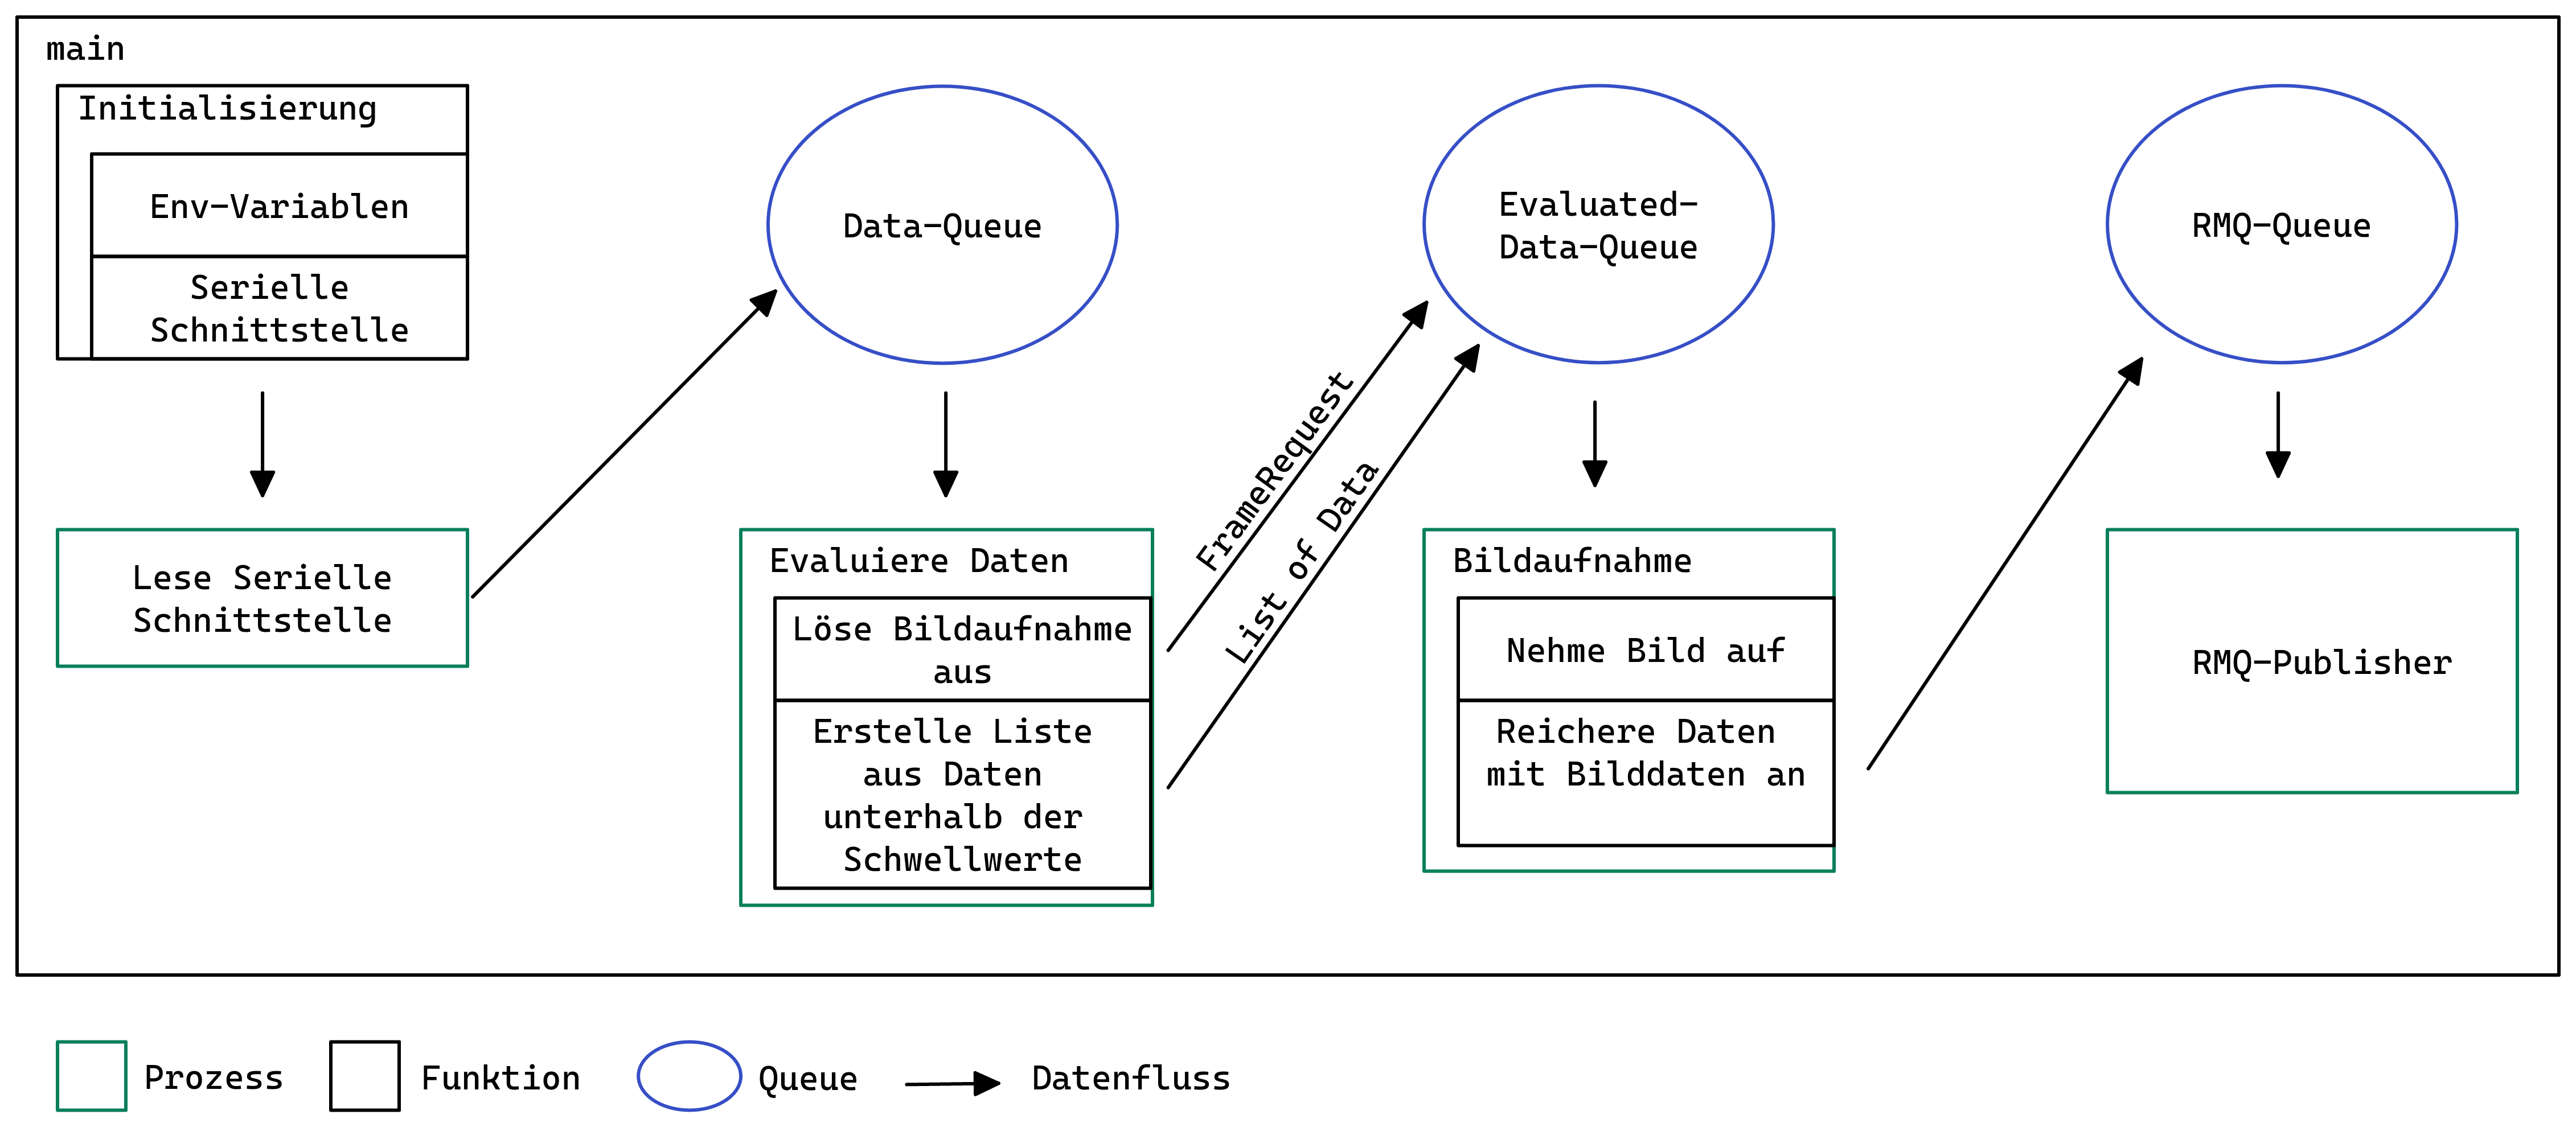
\includegraphics[width=1\textwidth]{pics/DataReaderDataFlow.png}
  \end{figure}
\end{frame}

\note[itemize]
{
  \item{Python}
  \item{Multiprocessing anstatt Multithreading wegen Gloabl Interpreter Lock}
  \item{4 parallele Prozesse}
  \item{Initialisierung}
  \item{Serieller Prozess}
  \item{Evaluierungs Prozess, FrameRequest, Schwellwert unterschreiten}
  \item{Bildaufnahme Prozess}
  \item{RabbitMQ-Publisher Prozess}
}


\begin{frame}[fragile]{Implementierung des Ausleseservice -- Pika}
  \begin{lstlisting}[style=MyPythonStyle,
    breaklines=true, firstnumber=75]
def rmq_sender(queue: Queue):
  config_reader = EnvConfig()
  config_reader.initialize_env()
  pub = Publisher(config_reader)
  pub.connect()
  site_id = config_reader.get_site_id()
  while True:
      try:
          if not queue.empty():
              data = queue.get()
              hyd_data = data_hydration(data, site_id)
              pub.publish(hyd_data)

          time.sleep(0.5)
      except Exception as ex: <@\\\large\vdots@>
\end{lstlisting}
\end{frame}

\note[itemize]
{
  \item{Beispiel RabbitMQ, also RMQ-Publisher}
  \item{Initialisierung}
  \item{Verbindungsdaten ueber Umgebungsvariablen}
  \item{Verbindung ueber Programmbibliothek Pika}
  \item{While schleife mit 500ms Abfrage}
}


\begin{frame}[fragile]{Implementierung des Datenspeicherservice}
  \begin{lstlisting}[style=bash-style,
    breaklines=true]
    Scaffold-DbContext "Data Source=sql-mar-01.druckhaus.local; Initial Catalog=PAMESAN; persist security info=True; user id=pamesan-rw; password=******" Microsoft.EntityFrameworkCore.SqlServer -OutputDir DatabaseContext -Tables RawData, ProcessedData
  \end{lstlisting}

  \note<1->[item]{C\#}
  \note<1->[item]{Database first Ansatz, Tabellen wurden vorher mit SQL erstellt}
  \note<1->[item]{EntityFrameworkCore}
  \note<1->[item]{DatenbankKontext und Tabellenmodelle werden automatisch erstellt}

  \pause

  \smartdiagramset{
    uniform color list=white for 4 items,
    uniform arrow color=true,
    arrow color=gray!50!black,
    back arrow disabled=true}
  \smartdiagram[flow diagram:horizontal]{Commit auf main-branch,
    GitLab Pipeline, Docker Image, Docker Swarm}

  \note<2->[item]{Deployment Prozess}
\end{frame}


\begin{frame}[fragile]{Implementierung des Datenspeicherservice}
  \begin{lstlisting}[style=cSharpStyle,
    breaklines=true, firstnumber=38]
internal static void SaveDataToRaw(string data, PAMESANContext dbContext) {
  try {
    RawData rawData = JsonConvert.DeserializeObject<RawData>(data)!;

    dbContext.RawData.Add(rawData);
    dbContext.SaveChanges();
  }
  catch {
      throw;
  }
}
\end{lstlisting}
\end{frame}

\note[itemize]
{
  \item{Code Beispiel fuer RawData}
  \item{Dependency Injektion Datenbankkontext}
  \item{Deserialisierung des JSON-Objekts}
  \item{Speichern in Datenbank}
  \item{Fehler zur Aufrufenden Methode durchreichen}
}


\begin{frame}[fragile]{Implementierung des Datenverarbeitungsservice}
  \vspace{0.7cm}
  \begin{minipage}[c][8cm]{\textwidth}
    \centering
    \smartdiagramset{
      uniform color list=white for 5 items,
      circular final arrow disabled=true,
      circular distance=2.25cm,
      arrow tip=to,
      arrow line width=2pt,
      uniform arrow color=true,
      arrow color=gray!50!black,
      additions={
          additional item bottom color=white,
          additional item border color=gray,
          additional item shadow=drop shadow,
          additional item offset=0.65cm,
          additional arrow line width=2pt,
          additional arrow tip=to,
          additional arrow color=gray!50!black,
        }
    }
    \smartdiagramadd[circular diagram]{
      Paketerkennung,Zuschnitt,Labelerkennung,Barcode auslesen,Paketgröße berechnen
    }{
      above of module1/RMQ-Subscriber,right of module5/RMQ-Publisher
    }
    \smartdiagramconnect{to-}{module1/additional-module1}
    \smartdiagramconnect{-to}{module5/additional-module2}
  \end{minipage}
\end{frame}

\note[itemize]
{
  \item{Datenverarbeitungsservice in Python}
  \item{RMQ-Subscriber fragen Daten ab}
  \item{Paketerkennung}
  \item{Bild entsprechend erkanntem Paket zuschneiden}
  \item{Labelerkennung mit OpenCV}
  \item{Barcode auslesen mit pyzbar}
  \item{Paketgröße berechnen}
  \item{Mit RabbitMQ publishen}
}


\begin{frame}[fragile]{Problemstellung Rollen und YOLOv7}
  \begin{minipage}[t]{0.49\textwidth}
    \begin{figure}[htpb]
      \centering
      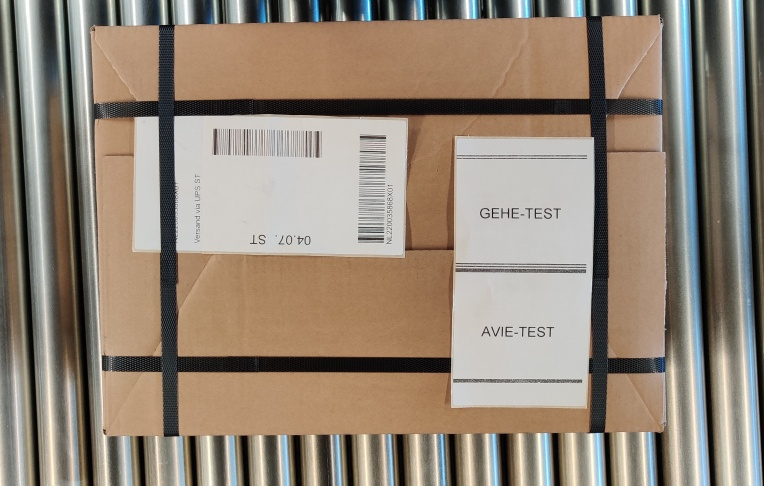
\includegraphics[angle=90,origin=c,width=0.8\textwidth]{pics/ShippingBox.jpg}
    \end{figure}

    \note<1->[item]{OpenCV, OpenComputerVision, Problem}
    \note<1->[item]{Spiegelende Rollen}
    \note<1->[item]{Loesung: Machine Learning}
  \end{minipage}
  \begin{minipage}[t]{0.49\textwidth}
    \pause
    \textbf{YOLOv7}
    \note<2->[item]{YOLOv7: You Only Look Once, Objektdetektor}
    \begin{itemize}
      \item Fully Convolutional Neural Network
            \note<2->[item]{FCNN: Neuronales Netzwerk, das nur aus Filtern besteht}
            \pause
      \item Erkennung von Objekten durch Semantische Segmentierung
            \note<3->[item]{Erkennung von Objekten durch Semantische Segmentierung -- Suche nach Bedeutung in Bildern, pixelweise}
            \pause
      \item Leichtes Training durch Bag of Freebies und Transfer Learning
            \note<4->[item]{Transfer Learning und Bag of Freebies: Methoden, die die Performance eines Modells erhöhen, ohne die Trainingszeit zu verlängern}
    \end{itemize}
  \end{minipage}
\end{frame}


\begin{frame}[fragile]{Labeln der Bilder}
  \begin{figure}[htpb]
    \centering
    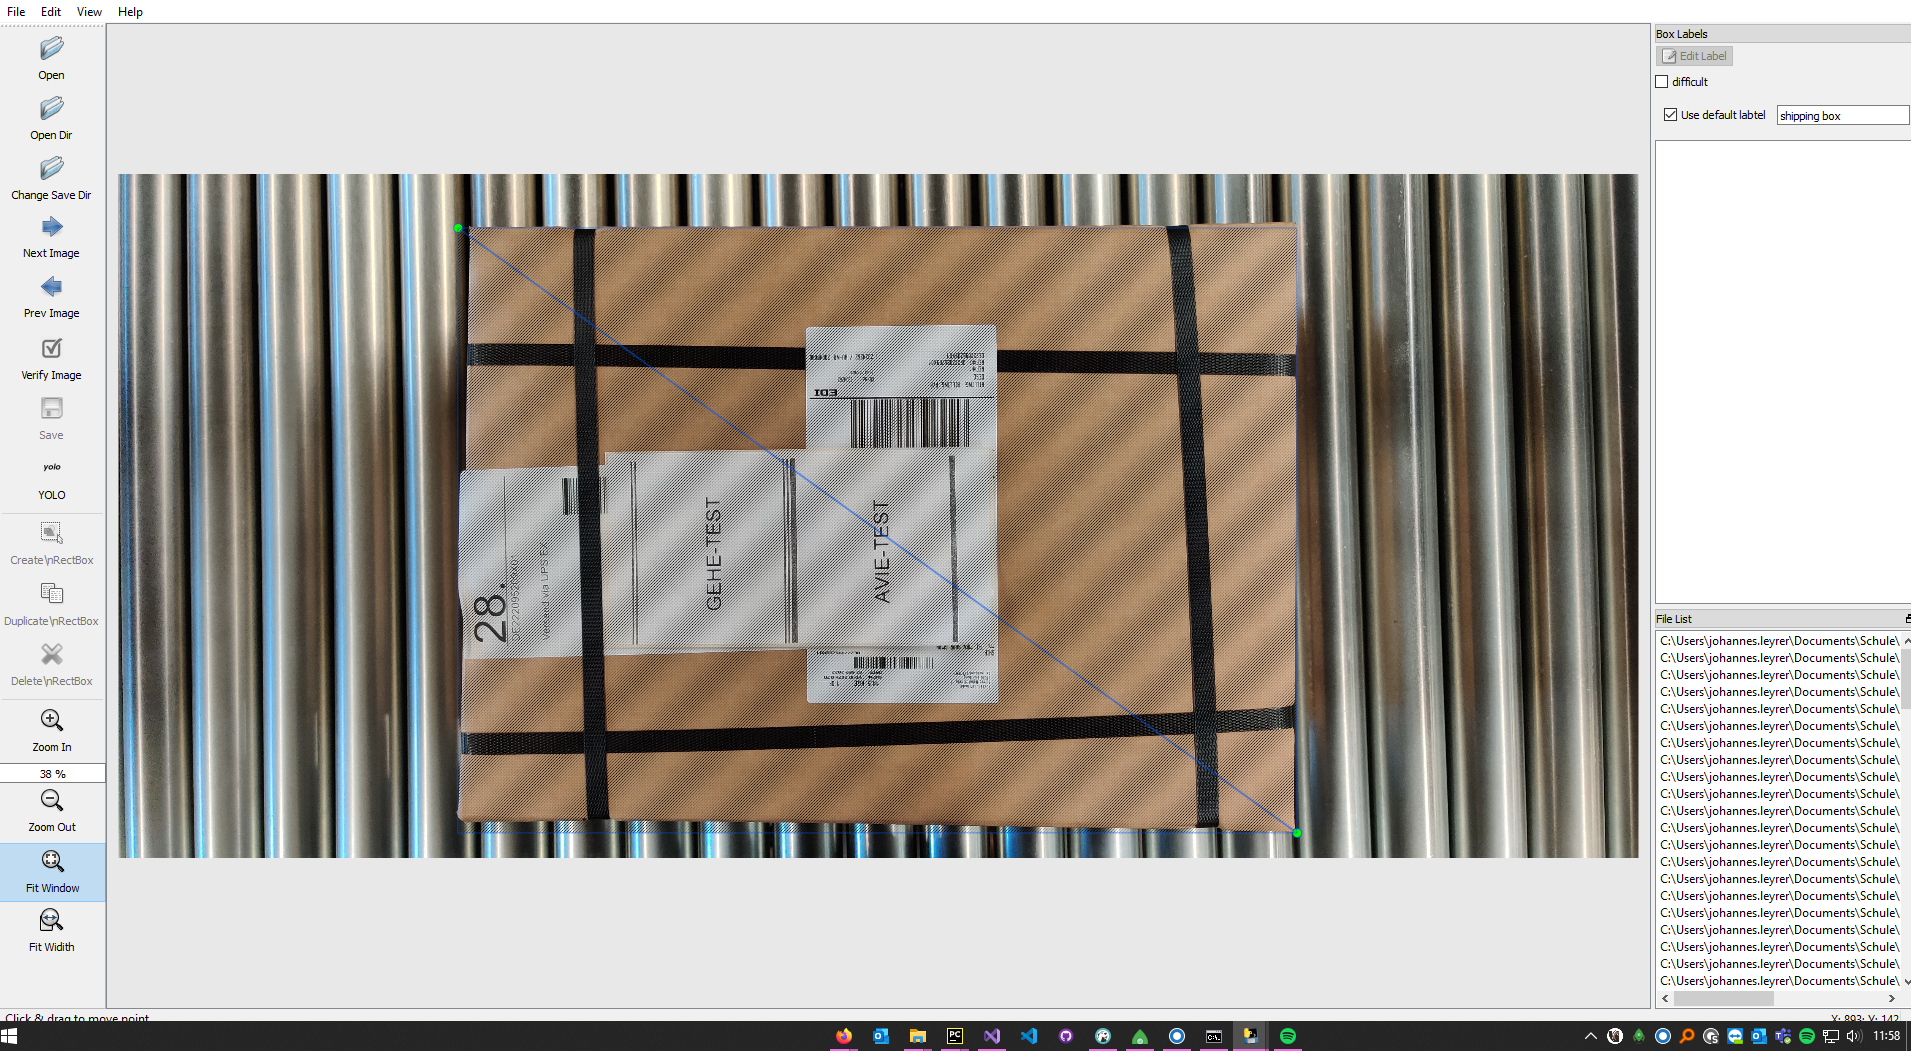
\includegraphics[width=1\textwidth]{pics/labelImg.png}
  \end{figure}
\end{frame}

\note[itemize]
{
  \item{Labeln der Bilder}
  \item{LabelImg}
  \item{100 Bilder}
}


\begin{frame}[fragile]{Training des YOLOv7-Models}
  \begin{lstlisting}[style=bash-style,
    breaklines=true]
    python train.py --device 0 --batch-size 16 --epochs 100 --img 640 640 --data data/custom_data.yaml --hyp data/hyp.scratch.custom.yaml --cfg cfg/training/yolov7_custom.yaml --weights yolov7.pt --name yolo7-custom
  \end{lstlisting}
\end{frame}

\note[itemize]
{
  \item{Datensatz in 80\% Trainingsdaten und 20\% Validierungsdaten aufteilen}
  \item{Traingsbefehl hier zu sehen}
  \item{batch size wie viele Bilder gleichzeitig}
  \item{100 Durchgaengen (--epochs) vor und zurueck}
}


\begin{frame}[fragile]{Ergebnis des YOLOv7-Models}
  \begin{figure}[htpb]
    \centering
    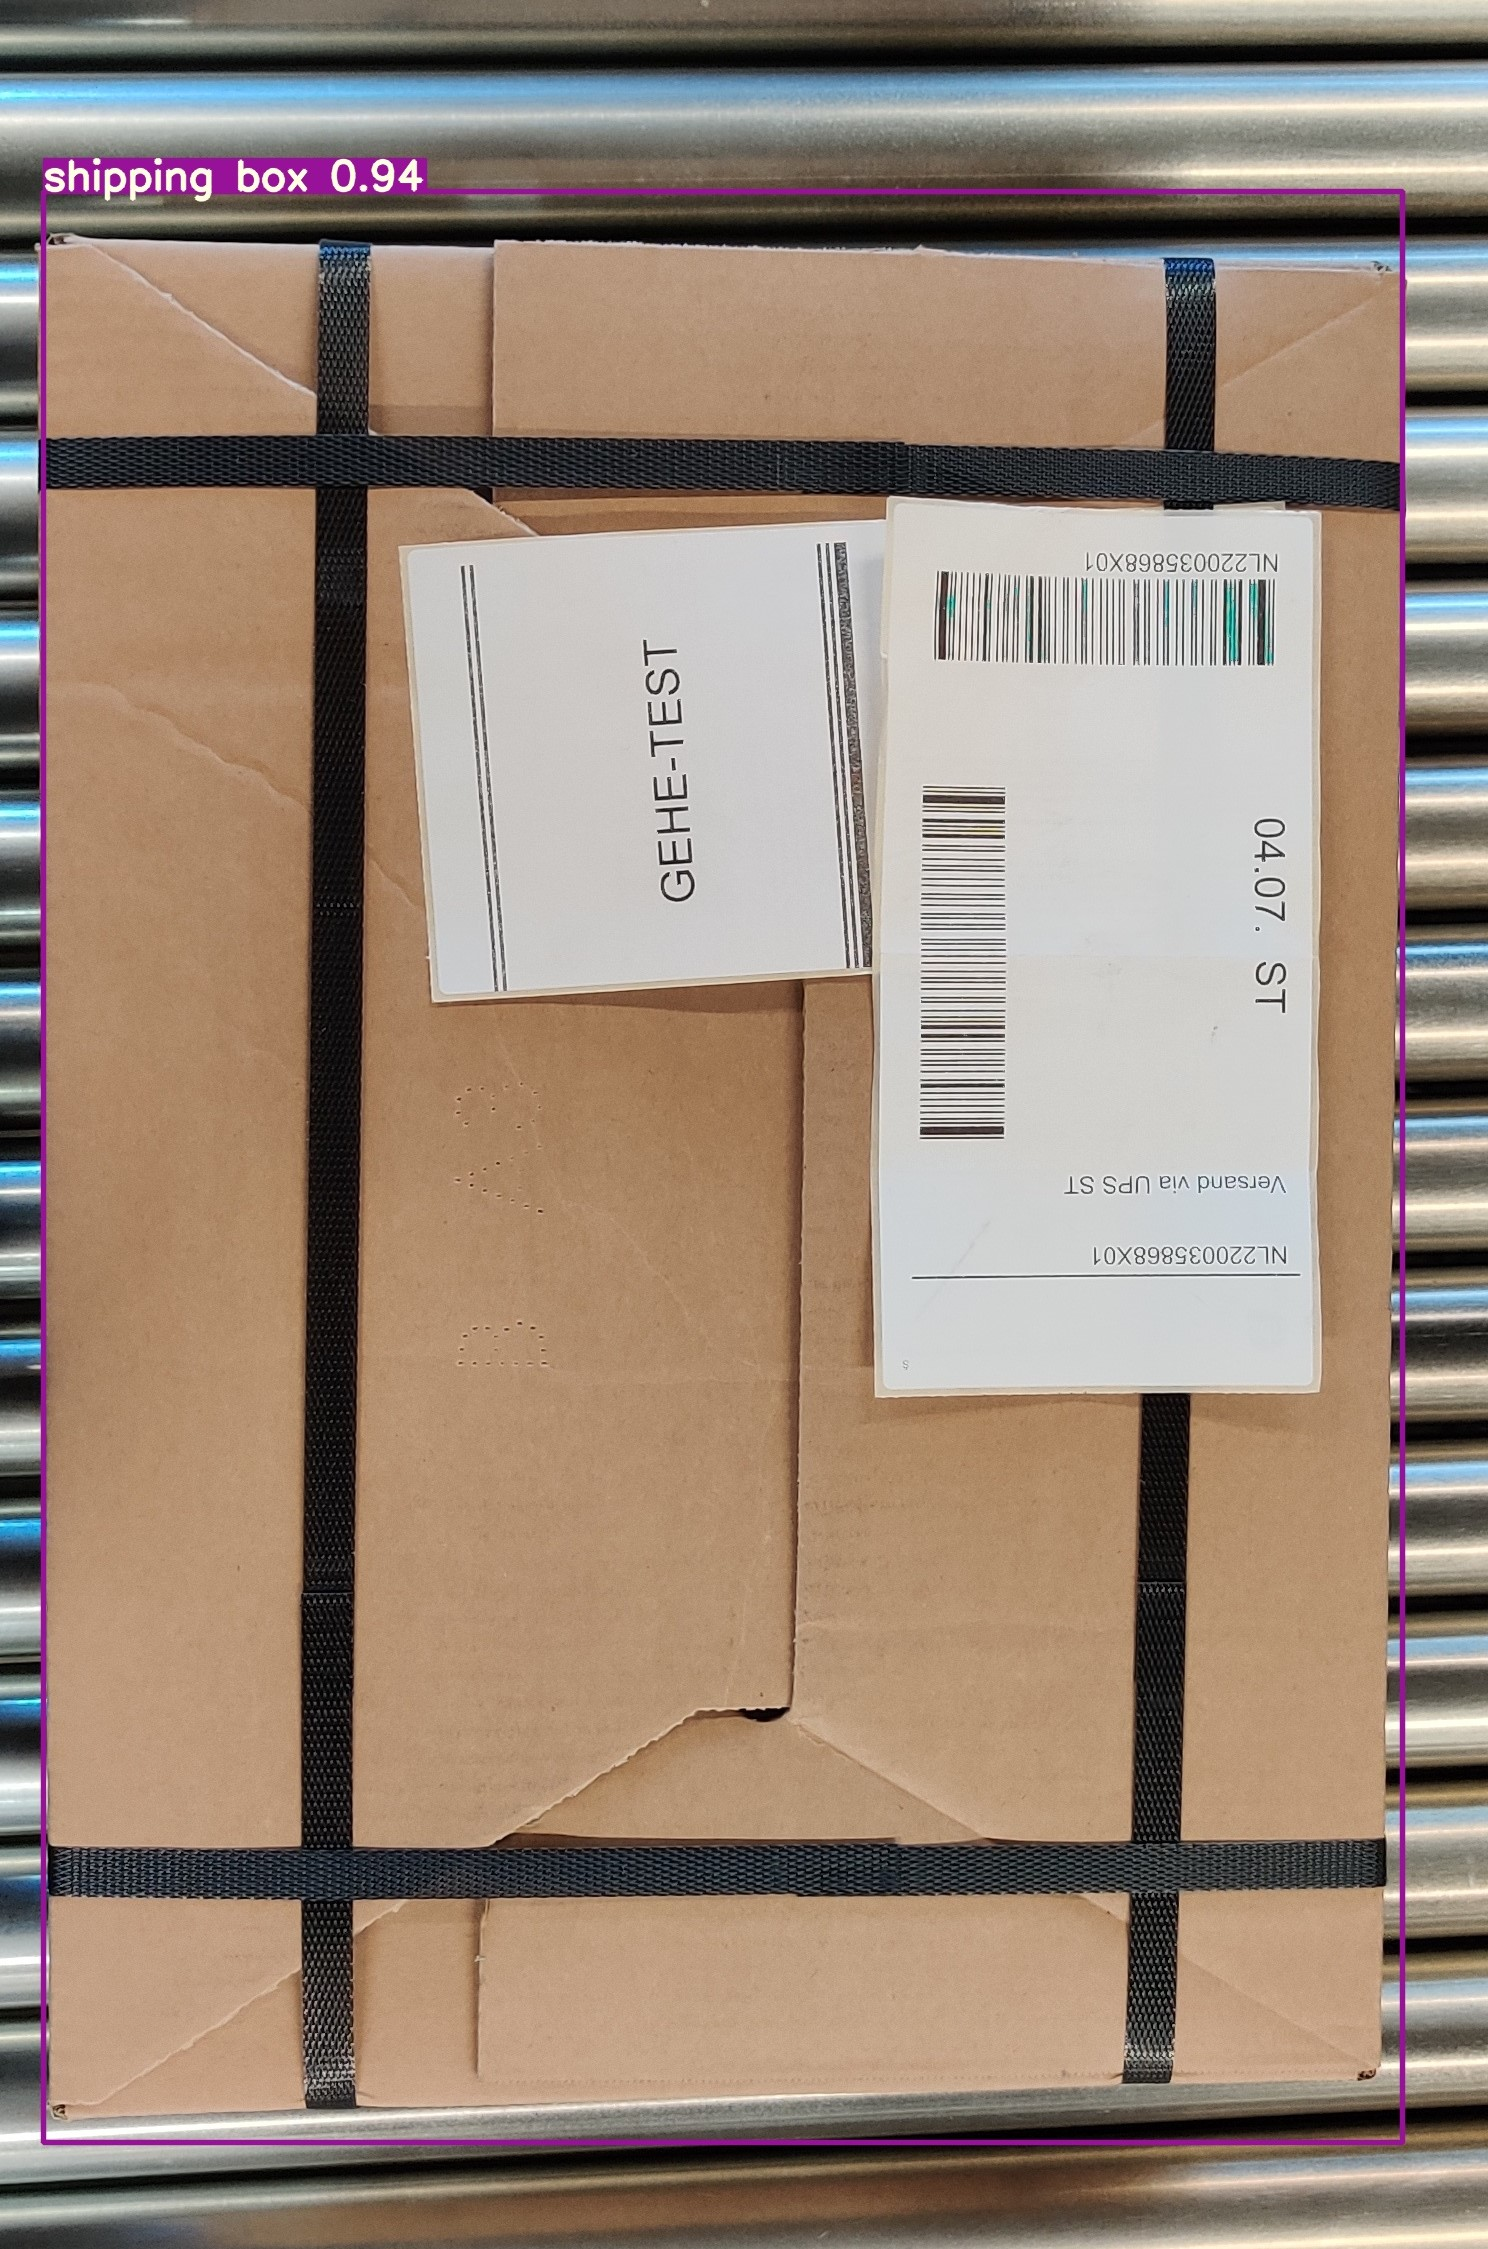
\includegraphics[angle=90,origin=c,width=1\textwidth]{pics/detectShippingBox.jpg}
  \end{figure}
\end{frame}

\note[itemize]
{
  \item{Ergebnis YOLOv7}
  \item{Model 94\% sicher, dass es ein Versandkarton ist}
  \item{Falls Zeit ist, MiniDemo nach der Praesentation}
}


\begin{frame}[fragile]{Auslesen des Versandlabels und Barcodes}
  \begin{figure}[htpb]
    \centering
    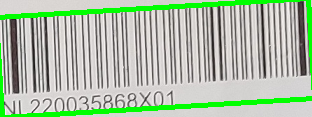
\includegraphics[width=1\textwidth]{pics/barcode.png}
  \end{figure}
\end{frame}

\note[itemize]
{
  \item{Versandlabelerkennung mit OpenCV}
  \item{Barcodeerkennung mit pyzbar}
}


\begin{frame}[fragile]{Berechnung der Paketgröße}
  \begin{lstlisting}[style=MyPythonStyle,
    breaklines=true, firstnumber=8]
def calculate_height(top_bottom: int, top_cm: int) -> int:
    return top_bottom - top_cm

def calculate_width(left_right: int, left_cm: int, right_cm) -> int:
    return left_right - left_cm - right_cm

def calculate_length(sensor_spacing: float, right_in: int, left_in: int, left_out: int) -> int:
    speed = sensor_spacing / (right_in - left_in)
    length = int((left_out - left_in) * speed)

    return length
  \end{lstlisting}
\end{frame}

\note[itemize]
{
  \item{Hoehe: Bekannter Abstand Sensor--Foerderband minus gemessener Abstand}
  \item{Breite: Bekannter Abstand der Sensoren minus gemessener Abstand}
  \item{Laenge: Berechnung durch Geschwindigkeit und bekannntem Versatz der seitlichen Sensoren}
}



\section{Fazit}
\begin{frame}[fragile]{Abschließender Zeitablauf}
  \begin{tikzpicture}

    \draw (0cm,0cm) -- (9.5cm,0cm);  %Abzisse
    \draw (0cm,0cm) -- (0cm,-0.1cm);  %linkes Ende der Abzisse
    \draw (9.5cm,0cm) -- (9.5cm,-0.1cm);  %rechtes Ende der Abzisse

    \draw (-0.1cm,0cm) -- (-0.1cm,5cm);  %Ordinate
    \draw (-0.1cm,0cm) -- (-0.2cm,0cm);  %unteres Ende der Ordinate
    \draw (-0.1cm,5cm) -- (-0.2cm,5cm) node [left] {h};  %oberes Ende der Ordinate

    \foreach \x in {10,20,...,40}  %Hilfslinien
    \draw[gray!50, text=black] (-0.2 cm,\x * 0.1 cm) -- (9.5 cm,\x * 0.1 cm)
    node at (-0.5 cm,\x * 0.1 cm) {\x};  %Beschriftung der Hilfslinien

    \node at (4.5cm,5.5cm) {Abschließender Zeitablauf};  %Überschrift

    \foreach \x/\y/\country in {0.5/10/Analyse,  %\x ist Anfang der Säulen
        2/8/Entwurf,  %\y ist Höhe der Säulen
        3.5/39/Implementierung,
        5/5/Test,
        6.5/6/Einführung,
        8/12/Dokumentation}
      {
        \draw[fill=mSybilaRed] (\x cm,0cm) rectangle (0.5cm+\x cm,\y * 0.1 cm) %die Säulen
        node at (0.2cm + \x cm,\y * 0.1 cm + 0.3cm) {\y}; %die Prozente über den Säulen
        \node[rotate=45, left] at (0.6 cm +\x cm,-0.1cm) {\country}; %Säulenbeschriftung
      };

    \foreach \x/\y in {0.9/10,  %\x ist Anfang der Säulen
        2.4/8,  %\y ist Höhe der Säulen
        3.9/46,
        5.4/2,
        6.9/2,
        8.4/12}
      {
        \draw[fill=darkgreenshade] (\x cm,0cm) rectangle (0.5cm+\x cm,\y * 0.1 cm) %die Säulen
        node at (0.25cm + \x cm,\y * 0.1 cm + 0.3cm) {\y}; %die Prozente über den Säulen
      };

    \draw[fill=mSybilaRed] (7cm,4.5cm) rectangle (7.2cm,4.7cm) node at (8cm,4.6cm) {h geplant};
    \draw[fill=darkgreenshade] (7cm,4cm) rectangle (7.2cm,4.2cm) node at (8.2cm,4.1cm) {h gebraucht};

  \end{tikzpicture}
\end{frame}

\note[itemize]
{
  \item{Abschließender Zeitablauf}
  \item{Anfangs gut}
  \item{Implementierung durch Paketerkennung verzoegert}
  \item{Test und Einführung stark abgeschwaecht}
  \item{Dokumentation im Zeitplan}
}


\begin{frame}[fragile]{Lessons Learned und Ausblick}
  \note<1->[item]{Was habe ich aus dem Projekt mitgenommen?}
  \textbf{Lessons Learned}
  \begin{itemize}
    \item YOLOv7 ist ein mit geringem Vorwissen leicht einsetzbarer Objektdetektor
          \note<1->[item]{YOLOv7 privat genutzt und gut einsetzbar}
          \pause
    \item Pufferzeit sollte \SI{2}{\percent} der Gesamtzeit betragen
          \note<2->[item]{Mehr Pufferzeit}
          \pause
    \item Industriekamera $>$ Webcam
          \note<3->[item]{Budget besser setzen, Industriekamera $>$ Webcam}
  \end{itemize}

  \pause

  \textbf{Ausblick}
  \note<4->[item]{Ausblick bzw. hier und jetzt}
  \begin{itemize}
    \item Verwendung KEYENCE-Scanner und Umschreiben auf C\#
          \note<4->[item]{KEYENCE, Umschreiben auf C\#, Wegfall von YOLOv7}
          \pause
    \item Verknüpfung erfasster Abmessungen mit bekannten Kartonagen
          \note<5->[item]{Gemessene mit Bekannte Kartonagen verknuepfen}
          \pause
    \item Aufbau an anderen Standorten
          \note<6->[item]{Aufbau an anderen Standorten}
  \end{itemize}
\end{frame}


\begin{frame}[standout]
  Fragen?
\end{frame}



\appendix


\begin{frame}[standout]
  Danke für die Aufmerksamkeit!
\end{frame}
\end{document}
